\documentclass[conference,letterpaper,10pt]{IEEEtran}
\usepackage{blindtext, graphicx, url, paralist}

% Add the compsoc option for Computer Society conferences.
%
% If IEEEtran.cls has not been installed into the LaTeX system files,
% manually specify the path to it like:
% \documentclass[conference]{../sty/IEEEtran}

% *** GRAPHICS RELATED PACKAGES ***
%
\ifCLASSINFOpdf
  % \usepackage[pdftex]{graphicx}
  % declare the path(s) where your graphic files are
  % \graphicspath{{../pdf/}{../jpeg/}}
  % and their extensions so you won't have to specify these with
  % every instance of \includegraphics
  % \DeclareGraphicsExtensions{.pdf,.jpeg,.png}
\else
  % or other class option (dvipsone, dvipdf, if not using dvips). graphicx
  % will default to the driver specified in the system graphics.cfg if no
  % driver is specified.
  % \usepackage[dvips]{graphicx}
  % declare the path(s) where your graphic files are
  % \graphicspath{{../eps/}}
  % and their extensions so you won't have to specify these with
  % every instance of \includegraphics
  % \DeclareGraphicsExtensions{.eps}
\fi

\usepackage{microtype}

\usepackage[tight,footnotesize]{subfigure}
\usepackage{fixltx2e}

\usepackage{multirow}

\usepackage{algorithm2e}
\usepackage{algorithm,algorithmic}
\usepackage{xcolor}
\newcommand\todo[1]{\textcolor{red}{#1}}

\hyphenation{op-tical net-works semi-conduc-tor}

\newtheorem{definition}{\textbf{Definition}}[section]
\newtheorem{theorem}{\textbf{Claim}}[section]
\newtheorem{corollary}{\textbf{Corollary}}[theorem]
\newtheorem{lemma}[theorem]{\textbf{Lemma}}

\begin{document}

\title{Tunnels to Towers: Secure Virtual Private Networking for CCN}


\maketitle


\begin{abstract}
Content Centric Networking (CCN) is a future Internet architecture which is envisioned as an alternative to the current IP-based model. CCN emphasizes content distribution by making contents directly addressable in a request-based information centric network. An advantage of CCN is that it has some innate privacy friendly features, such as lack of source and destination addresses in packets. However, to be considered a viable future Internet architecture, CCN must offer services for private and anonymous communication that are at least equivalent for  to those present in the IP architecture. Among such, VPNs are a very popular application that enables users to send and receive data across shared or public networks as if their computing devices were directly connected to the same private network. In this work we design, implement and evaluate CCVPN, a content centric virtual private network capable of providing the same functionality of VPNs within the CCN Internet architecture. To the best of our knowledge CCVPN is the first proposal of a VPN alike service for CCNs. In addition to the CCVPN design, we also provide a security analysis and experimental performance evaluation for this new system.
\end{abstract}

\begin{IEEEkeywords}
%Human Mobility, Group Detection, Group Dynamics, Periodicity, Opportunistic Routing.
\end{IEEEkeywords}

\IEEEpeerreviewmaketitle

\section{Introduction}
Content-centric networking (CCN) is a type of request-based information-centric
networking (ICN) architecture. In CCN, all data is named. Consumers obtain data
by issuing an explicit request for the content by its name. The network is
responsible for forwarding this request towards producers, based on the name,
who then generate and return the content response. Since a name uniquely identifies
a content response, routers may cache these packets to use in response to
future requests for the same name. As a consequence, all content has an (implicit
or explicit) authenticator that is used to verify the name-to-data binding. In
order to prevent cache poisoning attachs, wherein a malicious producer supplies
fake data in a content response that is propogated in the network, a router
should never serve (a) content with an invalid authenticator or (b) cached
content that it cannot verify. To enable (b), content objects with a digital
signature are expected to carry the public verification key or certificate. If the
authenticator is a MAC, then intermediate routers cannot verify it and should
therefore not cache the content.

One negative side effect of name-based requests is that any on-path or
eavesdropping adversary between a consumer and producer can learn the identity
and contents of all data in transit. In traditional IP-based networks, there are
generally two types of mechanisms to solve this problem: (1) anonymity
networks such as Tor \cite{tor} or (2) VPNs. As tools focused on anonymity,
the former help prevent linkability of packets to their requestors without
always protecting the identities or content themselves. In contrast, VPNs focus
on packet confidentiality by creating a tunnel between two private networks
or a consumer and single private network. All traffic over this tunnel is
encrypted and thereby opaque to an eavesdropper. VPNs differ from anonymity
networks such as Tor in that they are \emph{network-layer} mechanisms that
typically only introduces a single layer of encryption to protect traffic.
Thus, while Tor can be used to enable VPN-like functionality, it is often
far more inefficient since it operates above the network layer.

In ICN (or more specifically, CCN and NDN), ANDaNA was the first anonymity network of its
kind. Similar to Tor, ANDaNA uses circuits formed from anonymizing routers (ARs)
to marshall requests and responses between consumers and producers. The former
onion-encrypt interests and content using the public key(s) of the target ARs.
A variant of ANDaNA uses symmetric keys for packet encapsulation but suffers from
linkability. Tsudik et al. \cite{tsudik2016ac3n} proposed an optimized version of the symmetric-key
ANDaNA variant that did not permit linkability. To the best of our knowledge, there
is no anonymity network variant for ICN architectures. Though tunneling is only
useful for only a subset of ICN traffic, we believe it is a gap to be addressed
for this emerging technology, for a variety of reasons. {\bf First}, privacy
continues to be an elusive property for CCN applications. Tunneling will help
permit some degree of privacy within trusted AS domains from external passive
eavesdroppers. {\bf Second}, multi-hop circuits as used in ANDaNA are overkill
when trying to retain privacy instead of anonymity. {\bf Third}, end-to-end
sessions such as those enabled by CCNxKE \cite{ccnxke} and similar protocols
only serve those engaged in the session. In contrast, since the threat model is
different, tunneled traffic has the potential to serve any number of consumers
within the same trusted domain. Thus, while tunneling may contrast the content-centric
nature of data transmission in CCN, it fills a needed void for this architecture.

In this paper, we present CCVPN, a secure tunneling protocol and system design for
CCN. Similar to ANDaNA, CCVPN encrypts interests and content objects between producers
and consumers. In contrast, CCVPN only encrypts packets between a \emph{single}
source and destination to form a tunnel. In the standard configuration, both
endpoints of the tunnel are gateways between two trusted domains. It is possible,
however, for the source to be an individual consumer. In fact, the standard two-hop
ANDaNA circuit is identical to a nested tunnel with the same source. Thus,
CCVPN is more flexible than a general anonymity network.

The rest of this paper is organized as follows. Section \ref{sec:prelims} provides
an overview of CCN and the relevant protocol details necessary to understand
CCVPN. Section \ref{sec:related} describes previous related work that motivates
our design. Section \ref{metho} then describes the main CCVPN design with the necessary
cryptographic and packet format details. We analyze the security of CCVPN
in Section \ref{sec:sec-analysis}. We present the results of a comprehensive
analysis and experimental evaluation in Sections \ref{sec:analysis} and \ref{sec:exp},
respectively. We then conclude with a discussion of future work in Section \ref{sec:conclusion}

\section{Preliminaries}
This section presents an overview of the CCN architecture\footnote{Named-Data Networking \cite{jacobson2009networking}
is an ICN architecture related to CCN. However, since CCNxKE was
designed for ICNs that have features which are not supported by NDN (such
as exact name matching), we do not focus on NDN in this work. However,
CCNx could be retrofitted to work for NDN as well.} and work
related to confidentiality, privacy, and transport security. Those familiar with these topics
can skip it without loss of continuity.

\subsection{CCN Overview}
In contrast to IP networks, which focus on end-host names and addresses,
CCN \cite{jacobson2009networking,mosko2016semantics} centers
on content by making it named, addressable, and routable within the network. A
content name is a URI-like string composed of one or more
variable-length name segments, each separated by a \url{`/'} character. To
obtain content, a user (consumer) issues a request, called an \emph{interest}
message, with the name of the desired content. This interest can be
\emph{satisfied} by either (1) a router cache or (2) the content producer. A
\emph{content object} message is returned to the consumer upon satisfaction of
the interest. Moreover, name matching in CCN is exact, e.g., an interest for
\url{/edu/uci/ics/cs/fileA} can only be satisfied by a content object
named \url{/edu/uci/ics/cs/fileA}.

In addition to a payload, content objects include several fields. In this work,
we are only interested in the following three: {\tt Name}, {\tt Validation}, and {\tt ExpiryTime}.
The {\tt Validation} field is a composite of (1) validation algorithm information
(e.g., the signature algorithm used, its parameters, and a link to the public
verification key), and (2) validation payload (e.g., the signature). We use the
term ``signature'' to refer to this field. {\tt ExpiryTime} is an optional,
producer-recommended duration for the content objects to be cached.
Conversely, interest messages carry a mandatory name, optional payload, and
other fields that restrict the content object response. The reader is encouraged
to review \cite{mosko2016semantics} for a complete description of all packet fields
and their semantics.

Packets are moved in the network by routers or forwarders. A forwarder is composed
of at least the following two components:
\begin{compactitem}
\item {\em Forwarding Interest Base} (FIB) -- a table of name prefixes and
  corresponding outgoing interfaces. The FIB is used to route interests based on
  longest-prefix-matching (LPM) of their names.
\item {\em Pending Interest Table} (PIT) -- a table of outstanding (pending)
  interests and a set of corresponding incoming interfaces.
\end{compactitem}
%
A forwarder may also maintain an optional {\em Content Store} (CS) used for content
caching. The timeout for cached content is specified in the \texttt{ExpiryTime}
field of the content header. From here on, we use the terms {\em CS} and
{\em cache} interchangeably.

Forwarders use the FIB to move interests from consumers towards producers and the PIT
to forward content object messages along the reverse path towards consumers. More
specifically, upon receiving an interest, a router $R$ first checks its cache
(if present) to see if it can satisfy this interest locally. If the content is
not in the cache, $R$ then consults the PIT to search for an outstanding
version of the same interest. If there is a PIT match, the new incoming interface
is added to the PIT entry. Otherwise, $R$ forwards the interest to the next hop
according to its FIB (if possible). For each forwarded interest, $R$ stores
some amount of state information in the PIT, including the name of the interest and the
interface from which it arrived, so that content may be sent back to the
consumer. When content is returned, $R$ forwards it to all interfaces listed in
the matching PIT entry and said entry is removed. If a router receives a content object
without a matching PIT entry, the message is deemed unsolicited and subsequently
discarded.

\section{Related Work} \label{sec:related}

There are generally two classes of related work: (1) anonymity networks, such
as ANDaNA \cite{dibenedetto2011andana} and AC3N \cite{tsudik2016ac3n}, and
(2) encryption-based access control techniques. ANDaNA was developed as a
proof-of-concept application-layer anonymizing network for NDN. It works by
creating single-use, ephemeral, and anonymizing circuits between a consumer
and producer. Each hop in this circuit uses onion decryption to decapsulate
interests and onion encryption to encrypt the result. A minimum of two hops are
needed to guarantee consumer and producer unlinkability. CCVPN seeks to address
a different threat: privacy instead of anonymity. Thus, only a single hop, which
creates a tunnel between a source and a sink AS, is needed in CCVPN. Moreover,
since these tunnels serve multiple traffic flows for \emph{all} consumers within
the same source, they are long-lived and persistent. This reduces the per-packet
and per-flow cryptographic operations needed to move packets between the source
and sink domains. AC3N \cite{tsudik2016ac3n} is an optimized version of ANDaNA
that keeps per-flow state in each hop of an anonymizing circuit to specify
ephemeral key identifiers for packets. This prevents intra-flow linkability
while simultaneously enabling symmetric-key encryption and decryption for more
efficient processing. However, since AC3N is still a per-consumer application,
anonymizing circuits cannot be shared among multiple geolocated consumers
in the same domain.

Content encryption seeks to solve the problem of data confidentiality rather than
privacy or anonymity. This technique allows content to be disseminated throughout
the network, since it cannot be decrypted by adversaries without the appropriate decryption key(s).
Many variations of this approach have been proposed based on general
group-based encryption \cite{Smetters2010}, broadcast encryption \cite{Misra2013,Ion2013}, and
proxy re-encryption \cite{Wood2014}. Kurihara et al. \cite{ifip15} generalized these specialized
approaches in a framework called CCN-AC, an encryption-based access control framework
that shows how to use manifests to explicitly specify and enforce other encryption-based
access control policies. Consumers use information in the manifest to (1) request appropriate
decryption keys and (2) use them to decrypt content object(s). The NDN NBAC \cite{yu2015name}
scheme is similar to \cite{ifip15} in that it allows decryption keys to be
flexibly specified by a data owner. However, it does this based on name engineering rules instead of
configuration. Interest-based access control \cite{ghali2015interest} is a different
type of access control scheme wherein content is optionally encrypted. Access
is protected by making the names of contents derivable only by authorized consumers.
NDN-ACE \cite{shangndn} is a recent access control framework for IoT environments
which includes a key exchange protocol for distributing secret keys to sensors.
All of these techniques, with few exceptions, use public-key cryptographic schemes
to protect only the \emph{payload} of content packets. They do not encapsulate complete
packets for private transmission between a source and sink domain. The exception is CCNxKE~\cite{ccnxke},
which specifies a key exchange protocol that can bootstrap secure sessions between a source
a sink. CCNxKE can be used by CCVPN to establish pairwise shared secrets between tunnel
endpoints, even though this step is not strictly required.

\section{CCVPN}\label{metho}

Traditional Virtual Private Networks (VPNs) extend private networks across the Internet. They enable users to send and receive data across shared or public networks as if their computing devices were directly connected to the same private network~\cite{khanvilkar2004virtual}. The goal of CCVPN it to provide its users with the same functionality within the CCN Internet architecture. Therefore, the users can benefit from the features and security of a private network, even though the are not physically under the same private network.

\subsection{CCVPN Design}

In CCVPN, there are four main entities involved in the virtual private communication: \textit{Consumer}, \textit{Producer}, \textit{Consumer Side Gateway} ($G_c$), and \textit{Producer Side Gateway} ($G_p$). As in usual CCNs, the \textit{Consumer} is the network node that issues an interest for a given content (e.g., file, web page, video) that it wishes to retrieve. The Producer is the network node which originally created such content. $G_c$ and $G_p$ are the edge gateways responsible for ensuring the private communication among distinct domains. As we discuss later on, $G_c$ and $G_p$ can actually be implemented as a single network device, but we firstly present them as separate entities for the purpose of clarity.

\begin{figure*}[!ht]
\centering
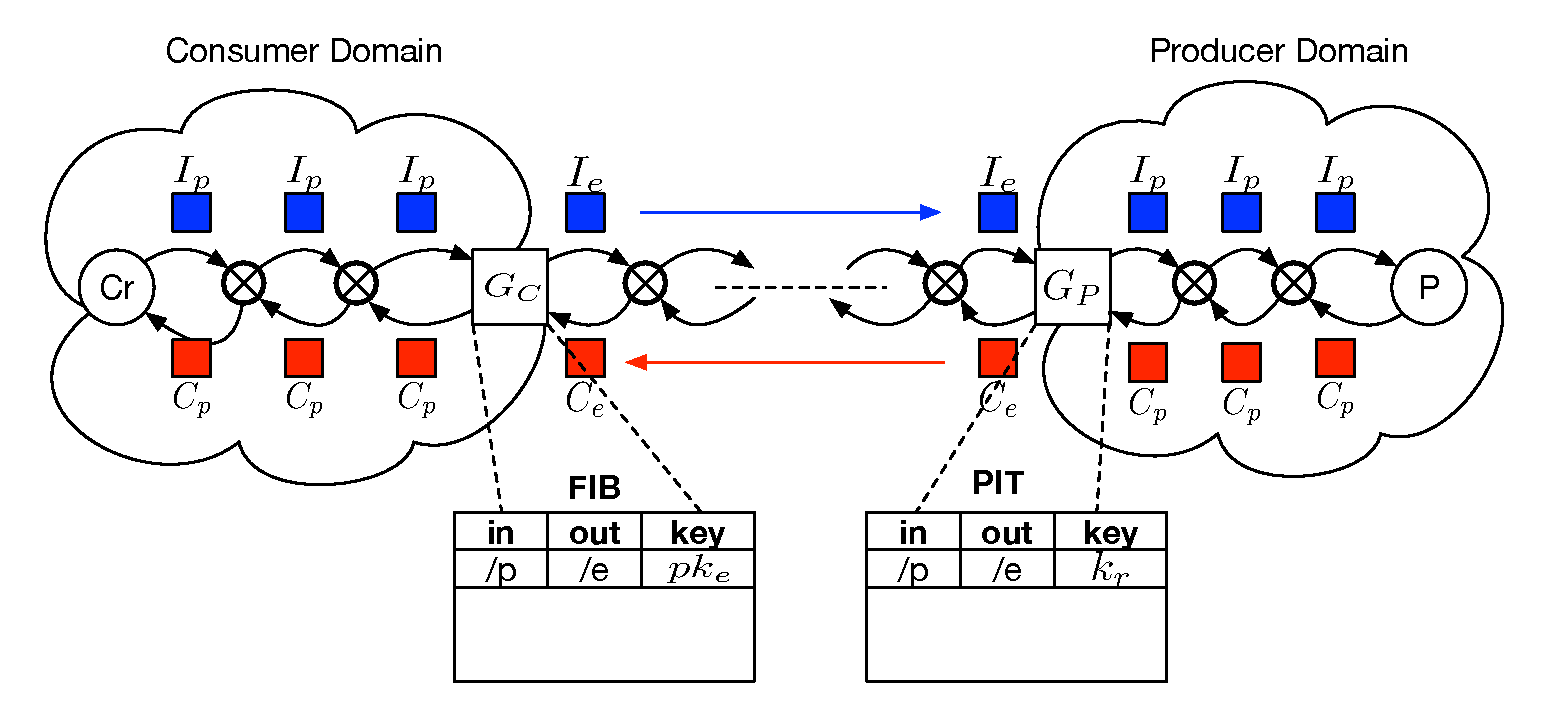
\includegraphics[width=1.9\columnwidth]{images/architecture.pdf}
\caption{CCVPN connectivity architecture}
\label{fig:ccvpn}
\end{figure*}

As depicted in Fig.~\ref{fig:ccvpn}, the devices inside the \textit{Consumer} domain form a physically interconnected private network. Conversely, the devices in the \textit{Producer} domain also form a private network. Therefore, the goal is to create an overlay virtual network that unifies the \textit{Consumer} and the \textit{Producer} domains in way such that the original interests and contents are only visible to the devices inside these two domains. In other words, the interest $I_e$ and the content $C_e$, that are forwarded outside these domains, should give no information about the original interest $I_p$ and the actual content $C_p$.

In order to achieve such anonymous communication, $G_c$ is introduced in the \textit{Consumer} domain to encapsulate outgoing interests. Conversely, the $G_p$ is responsible for decapsulating the incoming encapsulated interests and forwarding them in their original form. When the content is forwarded back in response to the interest, $G_p$ encrypts the content before sending it outside the \textit{Producer} domain. Finally, $G_c$ decrypts the received content to its original form and forwards it back towards the \textit{Consumer}. Through the rest of this section we provide a detailed description on how such actions are implemented.

Upon the arrival of a new interest $I_p$, $G_c$ checks its Forwarding Information Base (FIB) to check if the interest prefix is in the list of prefixes for VPN communication. We assume that the FIB must be pre-configured with the list of prefixes which will trigger the VPN communication. Associated with such prefixes are $G_p$'s name and public key ($pk_e$). Therefore, if the prefix of $I_p$ is in the VPN prefixes list, $G_P$ runs Algorithm~\ref{alg:interestEncap} to generate a new interest $I_e$ which encapsulates the original interest $I_p$. Firstly, Algorithm~\ref{alg:interestEncap} generates a random symmetric key ($k_r$) which will be used later on to perform the \textit{Content} Encryption/Decryption. Next, it retrieves $G_p$'s name and public key from the FIB. It uses the public key to encrypt the symmetric key $k_r$ and the original interest $I_p$. Then it creates the new interest $I_e$ with $G_p$'s name as the interest name and the generated ciphertext as payload. Since $I_e$ has  the $G_p$'s name it will be routed towards $G_p$ and since the payload is singed with $G_p$'s public key, only $G_p$ can retrieve the original interest $I_p$ and the symmetric key $k_r$.

\begin{algorithm}[]\label{alg:interestEncap}
\SetKwInOut{Input}{input}
\SetKwInOut{Output}{output}
\Input{Original interest $I_p$;}
\Output{Encapsulated interest $I_e$;}
%$Ip_{name}$ = getName($I_p$)\\
%storeToPIT($Ip_{name}$)\\
$k_r$ = symmKeyGen();\\
$Gp_{name}$ = retrieveNameFromFIB($I_p$)\\
$pk_e$ = retrievePKFromFIB($I_p$)\\
$payload$ = $Enc_{pk_e}(I_p||k_r)$\\
$I_e$ = createNewInterest($Gp_{name}$, $payload$)\\
storeToPIT($I_e$,$k_r$)\\
\Return $I_e$;\\
\caption{Interest encapsulation (runs on $G_c$)}
\end{algorithm}

After the message is routed towards $G_p$, $G_p$ verifies if the incoming interest name prefix matches its own name and, if it does, $G_p$ runs Algorithm~\ref{alg:interestDecap}, using its own secret key ($sk_e$) to decrypt $I_e$'s payload, which results in the original interest $I_p$ and the symmetric key $k_r$. $G_p$ then stores $I_e$'s name and the symmetric key $k_r$ in its own PIT, within the entry for the pending interest $I_p$, and forwards $I_p$. $I_e$'s name and $k_r$ are stored so that they can be used later on to generate the encrypted content $C_e$.

\begin{algorithm}[]\label{alg:interestDecap}
\SetKwInOut{Input}{input}
\SetKwInOut{Output}{output}
\Input{ Encapsulated interest $I_e$;}
\Input{ Private key $sk_e$;}
\Output{Original interest $I_p$;}
$Ie_{name}$ = getName($I_e$)\\
$cipherText$ = getPayload($I_e$)\\
$I_p||k_r$ = $Dec_{sk_e}(cipherText)$\\
storeToPIT($I_p$,$k_r$,$Ie_{name}$)\\
\Return $I_p$;\\
\caption{Interest decapsulation (runs on $G_p$)}
\end{algorithm}

The original interest $I_p$ is forwarded inside the \textit{Producer} domain until it reaches the \textit{Producer}. The \textit{Producer} responds with the content $C_p$ which is forwarded back to $G_p$.
Upon receiving $C_p$, $G_p$ fetches for $C_p$'s name (which is equal to $I_p$'s name) on its PIT, retrieving $k_r$ and $Ie$'s name. Then it uses $k_r$ to encrypt-then-MAC the real content response $C_p$ and creates $C_e$ which must have the same name as $I_e$ and the encryption of $C_p$ as payload (Algorithm~\ref{alg:contentEnc}). Since only $G_c$ and $G_p$ share the symmetric key $k_r$, only $G_c$ will be able to decrypt $C_e$'s payload into $C_p$. Therefore nobody from outside the VPN is able to access the content nor the Producer's identity.

\begin{algorithm}[]\label{alg:contentEnc}
\SetKwInOut{Input}{input}
\SetKwInOut{Output}{output}
\Input{Original content $C_p$;}
\Output{Encrypted content $C_e$;}
$name$ = getName($C_p$)\\
$k_r$ = retrieveKeyFromPIT($name$)\\
$Ie_{name}$ = retrieveNameFromPIT($name$)\\
$payload$ = $EncryptThenMAC_{k_r}(C_p)$\\
$C_e$ = createNewContent($Ie_{name}$,$payload$)\\
\Return $C_e$;\\
\caption{Content encryption  (runs on $G_p$)}
\end{algorithm}

Since $C_e$ and $I_e$ have the same name, $C_e$ will be forwarded all the way back to $G_c$. When $G_c$  receives $C_e$ $G_c$ will execute Algorithm~\ref{alg:contentDec}. It will match $C_e$'s name to the pending interest $I_e$ in its PIT, retrieving $k_r$. $k_r$ can then be used to verify the integrity of the received content and to decrypt it into the actual content $C_p$. After that, $C_p$ can be forwarded back to the \textit{Consumer}. If the MAC verification fails, it means that $C_e$ has been forged and $G_c$ ignores it.

\begin{algorithm}[]\label{alg:contentDec}
\SetKwInOut{Input}{input}
\SetKwInOut{Output}{output}
\Input{Encrypted content $C_e$;}
\Output{Original content $C_p$;}
$Ce_{name}$ = getName($C_e$)\\
$k_r$ = retrieveKeyFromPIT($Ce_{name}$)\\
$cipherText$ = getPayload($C_e$)\\
$C_p$ = Dec($k_r$,$cipherText$)\\
\eIf{$C_p$ == $\perp$}
    {
    \tcc{MAC verification failed}
    \Return ;\\
    }
    {\Return $C_p$;\\}
\caption{Content decryption (runs on $G_c$)}
\end{algorithm}

For clarity, we have defined a \textit{Consumer} and a \textit{Producer} domain. However, in reality, a single gateway can implement the functions of both $G_c$ and $G_p$. Therefore, consumers and producers can exist in both the domains and interests for contents can be issued from both sides. Also, it is worth to mention that, within the created CCVPNs, content caching would work just as it works in regular CCNs,  i.e., routers would be able to cache contents and respond to interests that were previously requested, enabling better resource usage and lower communication delays. Finally, we emphasize that $G_c$ encapsulation and decryption functions can also run inside the Consumer host. Conversely, $G_p$ can be implemented within the \textit{Producer} host. This enables its usage for one-to-one communication that would be completely anonymous to any  other entity in the network.

\subsection{System and Security Model}

Our security analysis considers the worst case scenario, in which the consumer issues an interest that has not been cached in any of the routers from the consumer nor producer domains. Therefore, the interest must traverse the whole network until reaching the content producer. Conversely, the content needs to be forwarded all the way back though the same path satisfying the routers' PIT entries. A system that is secure in this worst case is also secure when the content has been previously cached in some router along the way.

\textbf{Adversary Goals and Capabilities.} The goal of the adversary is either 1) to retrieve any information associated with the original issued interest $I_p$ and/or the original content $C_p$ or 2) to retrieve the identities of the consumer and/or producer, thus violating the anonymity in the communication. An adversary is also considered successful if it is able to impersonate the content producer by faking a content response. Since the original interest and the original content are visible inside the consumer and producer domains, we here assume that the adversary cannot eavesdrop or compromise hosts inside such domains. It is also worth to emphasize that, by the conceptual design of the VPN, communication is anonymous to hosts from outside the VPN but not to hosts that belong to that VPN. Anyhow, one-to-one anonymous communication is still achievable sing the VPN paradigm if the communication must be anonymous to any other host in the network\footnote{In the case that communication should be anonymous even to nodes inside the consumer and producer domains, $G_c$ and $G_p$ could be ran as processes within the consumer and producer hosts, respectively. This way, packets exchanged between them would remain anonymous to any other node in the network}. This also means that, as components of the producer and consumer domains, we assume that the gateways $G_c$ and $G_p$ cannot be compromised.

In our model the adversary is allowed to perform the following actions (when outside the consumer and producer domains):

\begin{itemize}
	\item \textbf{Eavesdrop and replay traffic:} An adversary can eavesdrop on a link learning among other things the packet contents and traffic patterns.
	\item \textbf{Deploy compromised routers or compromise existing routers:} An adversary is capable of deploying a compromised router ou compromised an existent router outside the VPN domains. By doing so the adversary becomes capable of maliciously injecting, delaying, altering, and dropping traffic. In addition, when an existing router is compromised, the adversary learns all of the private information contained in that router, such as private keys and cached content.
	\item \textbf{Deploy compromised caches:} As a consequence of the ability to compromise and deploy compromised routers, an adversary is also able to deploy compromised caches. This includes monitoring the routers' cache contents and replying with corrupted or fake data.
\end{itemize}

\subsection{Additional Considerations}

\textbf{Gateway-to-Gateway Authentication:} At this point one might have noticed that, in the CCVPN design, any host that possesses the producer -side gateway ($G_p$) public-key is able to initiate an anonymous communication link with $G_p$. In other words, the design does not include any authentication between the consumer-side gateway $G_c$ and $G_p$. Indeed, authentication is not required in CCVPN because is in not needed in some application scenarios.

Suppose, for instance, that a content provider offers its contents to any host in the Internet but it also  wants such hosts to be able to anonymously request and receive such content. In this case, since any host in the Internet should be able to requests the contents, there is no need for the consumer-side $G_c$ to authenticate it self to $G_p$.

Another use case for CCVPN is the traditional VPN use case, in which two physically separated local networks (for instances to offices of the same company in different countries) should virtually behave as a private local network. In that case, it is necessary to prevent that a given $G_c$, which is not part of that corporation's network to connect to $G_p$ and become part of the VPN. To that purpose, standard host-to-host CCN authentication mechanisms such as \cite{} can be used to authenticate $G_p$ and $G_c$ to each other. This must be performed before any VPN communication to make sure that only the appropriate parties are communicating under the CCVPN architecture. We discuss the evaluation and specification of gateway-to-gateway authetication protocols as future work (see Sec.~\ref{conclusion}).

\textbf{Denial of Service:} Since CCVPN gateways are connected to the public network they are clearly susceptible to DoS attacks. In the CCVPN architecture, both $G_c$ and $G_p$ are susceptible to DoS attacks. A DoS attack on $G_p$ would consist in flooding it with several fake encapsulated interests. Conversely, a DoS attack on $G_c$ would basically consist of flooding it with an enormous amount of encrypted content packets. In the case of $G_p$, such attacks are specially harmful since the interest decapsulation involves a public-key decryption operation.



\section{CCVPN Security}\label{sec:sec-analysis}


\subsection{System and Security Model} \label{sec:goals}

Our security analysis considers the worst case scenario, in which the consumer issues an
interest that has not been cached in any of the routers from the consumer nor producer domains.
Therefore, the interest must traverse the entire network until reaching the producer.
Conversely, the content needs to be forwarded all the way back though the same path
satisfying the routers' PIT entries. A system that is secure in this worst case is also
secure when the content has been previously cached in some router along the way.

\textbf{Adversary Goals and Capabilities.} The goal of the adversary \adv\ is either 1) to
retrieve any information associated with the original issued interest $I_p$ and/or the
original content $C_p$ or 2) to retrieve the identities of the consumer and/or producer,
thus violating the anonymity in the communication. \adv\ is also considered successful
if it is able to impersonate the content producer by faking a content response. Since the
original interest and the original content are visible inside the consumer and producer
domains, we here assume that \adv\ cannot eavesdrop or compromise hosts inside
such domains. It is also worth to emphasize that, by the conceptual design of the VPN,
communication is anonymous to hosts from outside the VPN but not to hosts that belong to
that VPN. Anyhow, one-to-one anonymous communication is still achievable sing the VPN
paradigm if the communication must be anonymous to any other host in the network. This
also means that, as components of the producer and consumer domains, we assume that the
gateways $G_c$ and $G_p$ cannot be compromised.

In our model \adv\ is allowed to perform the following actions (when outside the consumer and producer domains):

\begin{itemize}
	\item \textbf{Eavesdrop and replay traffic:} \adv\ can eavesdrop on a link
    learning among other things the packet contents and traffic patterns.
	\item \textbf{Deploy compromised routers or compromise existing routers:} \adv\ is capable of
    deploying a compromised router ou compromised an existent router outside the VPN domains. By doing
    so \adv\ becomes capable of maliciously injecting, delaying, altering, and dropping traffic.
    In addition, when an existing router is compromised, \adv\ learns all of the private
    information contained in that router, such as private keys and cached content.
	\item \textbf{Deploy compromised caches:} As a consequence of the ability to compromise and
    deploy compromised routers, \adv\ is also able to deploy compromised caches. This
    includes monitoring the routers' cache contents and replying with corrupted or fake data.
\end{itemize}

\subsection{Additional Considerations}

\textbf{Gateway-to-Gateway Authentication:} At this point one might have noticed that,
in the CCVPN design, any host that possesses the producer -side gateway ($G_p$) public-key
is able to initiate an anonymous communication link with $G_p$. In other words, the design
does not include any authentication between the consumer-side gateway $G_c$ and $G_p$.
Indeed, authentication is not required in CCVPN because is in not needed in some application scenarios.

Suppose, for instance, that a content provider offers its contents to any host in the Internet
but it also  wants such hosts to be able to anonymously request and receive such content. In
this case, since any host in the Internet should be able to requests the contents, there is no
need for the consumer-side $G_c$ to authenticate it self to $G_p$.

Another use case for CCVPN is the traditional VPN use case, in which two physically separated
local networks (for instance, offices of the same company in different countries) should virtually
behave as a private local network. In that case, it is necessary to prevent that a given $G_c$,
which is not part of that corporation's network to connect to $G_p$ and become part of the VPN.
To that purpose, standard host-to-host CCN authentication mechanisms can be used to authenticate
$G_p$ and $G_c$ to each other. This must be performed before any VPN communication, to make sure
that only the appropriate parties are communicating under the CCVPN architecture. We leave the
evaluation and specification of gateway-to-gateway authentication protocols as future work (see Sec.~\ref{sec:conclusion}).

\textbf{Denial of Service:} Since CCVPN gateways are connected to the public network they are
clearly susceptible to DoS attacks. In the CCVPN architecture, both $G_c$ and $G_p$ are
susceptible to DoS attacks. A DoS attack on $G_p$ would consist in flooding it with several
fake encapsulated interests. Conversely, a DoS attack on $G_c$ would basically consist
of flooding it with an enormous amount of encrypted content packets. In the case of $G_p$,
such attacks are specially harmful since the interest decapsulation involves a public-key
decryption operation. We plan to consider DoS countermeasures in future work.

\subsection{Security Analysis}

In this section we analyze the security of CCVPN. Our main security goal is
preventing \adv\ from achieving any of the goals outlined in Section \ref{sec:goals}.
Formally, this translates into semantic security of all traffic, modulo what can be inferred via traffic analysis.
A consequence of this property is that an off-path adversary, i.e., one that is
not in the consumer or producer domain, is unable to forge packets with
non-negligible probability. Our analysis relies on arguments in the standard
security model. It consists of assessing the security of the interest and
content encapsulation algorithms.

\begin{definition}\label{def1}
\textit{
An interest encapsulation algorithm $Encapsulate(I_p)$ is an indistinguishable
interest encapsulation iff, given any two interests $I_p^1$ and $I_p^2$, chosen
by the adversary, and a randomly selected bit $b$, the adversary has only $1/2 + \epsilon$
probability of guessing the value of the bit $b$ when given $I_e^b = Encapsulate(I_p^b)$.
Where $\epsilon$ is a negligible factor with regard to the security parameter $k$.
}
\end{definition}

\begin{theorem}\label{theo1}
\textit{
Let $Encapsulate_{pk}(I_p)$ denote the interest encapsulation routine described in
Algorithm~\ref{alg:interestEncap}. If $Enc_{pk}$, used to construct $Encapsulate_{pk}(I_p)$,
is a CPA-secure public-key encryption scheme then $Encapsulate_{pk}(I_p)$ is an
indistinguishable interest encapsulation algorithm.
}
\end{theorem}

\textit{\textbf{Proof--}} Suppose that Claim~\ref{theo1} is false. Then there exists a
polynomial adversary $Adv$ capable of guessing the bit $b$ of Definition~\ref{def1}
with non-negligible advantage, when given $I_e^b = Encapsulate(I_p^b)$ with
$b \leftarrow \{0,1\}$ chosen at random. We show that if such adversary exists he can
be used to construct a polinomial adversary $AdvCPA$ which breaks the CPA-security
of $Enc_{pk}$. $AdvCPA$ plays the CPA-security game with a challenger sending him
two messages $m^0$ and $m^1$. Following the CPA-security game, the challenger
randomly chooses a value for the bit $b' \leftarrow \{0,1\}$ and gives back
$C = Enc_{pk}(m^{b'})$ to $AdvCPA$. To break the CPA-security $AdvCPA$ must be
able to guess the value of the bit $b'$ with non-negligible advantage. To that
purpose $AdvCPA$ can query the challenger for the encryptions of $m^0$ and
$m^1$ ($c^0 = Enc_{pk}(m^0)$ and $c^1 = Enc_{pk}(m^1)$) and then construct two
interests $I_e^0 = createNewInterest(Gp_{name}, c^0)$ and $I_e^1 = createNewInterest(Gp_{name}, c^1)$,
using the same $createNewInterest$ function used by algorithm~\ref{alg:interestEncap},
which is public (notice that $Gp_{name}$ is also public). Finally, $AdvCPA$ gives $I_e^0$
and $I_e^1$ as input to $Adv$ and outputs whatever $Adv$ outputs. Since under our
assumption $Adv$ guesses the bit $b$ with non-negligible advantage, then $AdvCPA$ breaks
the CPA-security of $Enc_{pk}$. But this violates the hypothesis of Claim~\ref{theo1}
and, therefore, such $Adv$ cannot exist.

\begin{definition}
\textit{
A content encapsulation algorithm $Encapsulate(C_p)$ is an indistinguishable content
encapsulation iff, given any two contents $C_p^1$ and $C_p^2$, chosen by the adversary,
and a randomly selected bit $b$, the adversary has only $1/2 + \epsilon$ probability
of guessing the value of the bit $b$ when given $C_e^b = Encapsulate(C_p^b)$. Where
$\epsilon$ is a negligible factor with regard to the security parameter $k$.
}
\end{definition}

\begin{theorem}
\textit{
Let $ContentEnc_{k_r}(C_p)$ denote the content encapsulation routine described in
Algorithm~\ref{alg:contentEnc}. If $EncryptThenMAC_{k_r}$, used to construct
$ContentEnc_{sk}$, is a CCA-secure symmetric-key encryption scheme, then:
\begin{enumerate}
\item $ContentEnc_{k_r}(C_p)$ is an indistinguishable content encapsulation algorithm;
\item An adversary has only negligible probability of generating a valid fake encapsulated content $I_c'$
\end{enumerate}
}
\end{theorem}

\textit{\textbf{Proof (Sketch)--}} This follows directly from the definition of
CCA-security and from the same argument in the previous proof.

\section{Performance Analysis}\label{sec:analysis}

In this section we analyze and discuss the overhead of the CCVPN design with respect
to the additional processing time and state consumption needed to handle traffic.

\subsection{State Consumption}
The CCVPN design has an immediate impact on the FIB and PIT size of a gateway.
(The content store size remains unaffected since only decapsulated content objects
are ever cached.) Let $F_S$ be the total size of a standard forwarder
FIB in terms of bytes and
$N_F$ be the number of entries in the FIB. For simplicity, we will assume that
each name prefix in the FIB has a constant size of $64$B. In practice we expect
this to be a comfortable upper bound. Thus, $F_S = N_Fs$, where $s$ is the size of
each FIB entry. Here, $s$ includes a name prefix (of size $64$B) and a bit vector
that identifies the matching links for the interface. We assume that a gateway has
$128$ links which, again, is a comfortable upper bound. Therefore, $F_S = 80N_F$B.
Now consider the FIB size $F_G$ for a CCVPN gateway. Some entries in these FIBs will
point to ``private'' prefixes, i.e., other domains, and therefore have a larger size
to account for the corresponding prefix and key material that must be stored.
For both public- and symmetric-key encryption, the key size is the same: $32$B \cite{sodiumGithub}. 
Therefore, by taking into account two both the FIB entry prefix key, translation
prefix, encryption key, and corresponding bit vector, the total size of one ``private''
FIB entry will be $176$B, meaning that $F_G = 176N_F$B. By comparing $F_S$ to $F_G$, we
see that, in the worst case, the CCVPN FIB is at most $F_G/F_S = 176/80 = 2.2$ times larger
than the standard FIB. In practice, however, we expect this to be much smaller, since the
fraction of public to private FIB entries in a gateway will be non-zero.

We will now apply the same analysis to the PIT size. A standard PIT entry includes a
complete name and ingress bit vector. (They may also include the optional {\tt KeyId}
and {\tt ContentId}, but since they are included in the gateway PIT as well we omit them
from this analysis.) A gateway PIT entry will contain the same elements of a standard
PIT entry but also a symmetric encryption key ($32$B), nonce ($12$B), and an
encapsulation name ($64$B + $32$B).
The encapsulation name is the name of an encapsulated interest and includes an additional
$32$B {\tt PayloadID} segment to identify the encapsulated value in the payload. Let
$P_S$ and $P_G$ be the sizes of the standard and gateway PIT, respectively, and let $N_P$
be the number of PIT entries in one such table. Based on the above discussion, and assuming
again that a name is at most $64$B, a standard PIT entry is of the size $80$B. In contrast,
a gateway PIT entry is of size $204$B. Therefore, in the worst case, the CCVPN PIT
will be at most $P_G / P_S = 204/80 = 2.55$B larger than the standard PIT. Assuming
a steady state size of approximately $1e^5$ entries \cite{carofiglio2015pending},
this means that the PIT will be $20.4$MB, which is well within the capacity of
modern memory systems.

\subsection{Processing Overhead}
In terms of processing overhead, the gateway adds a number of new steps to the data
path of a packet. The main computational burdens are packet encapsulation and decapsulation.
In the public-key variant of CCVPN, interests are processed using public-key encryption,
whereas content is always processed using symmetric-key encryption. Let $T_E^P(n)$ and $T_D^P(n)$
be the time to encrypt and decrypt $n$B of data using a suitable public-key encryption scheme.
Similarly, let $T_E^S(n)$ and $T_D^S(n)$ be the time to encrypt and decrypt $n$B of data
using a symmetric-key encryption scheme. Then, the latency in a single interest-content
exchange is increased by $T = T_E^P(n_I) + T_D^P(n_I) + T_E^S(n_C) + T_D^S(n_C)$, where
$n_I$ and $n_C$ are the original interest and content sizes, respectively. As a rough
estimate, \cite{benchmarks} lists the cost of AES-GCM to be $2.946\mu s$ for setup
followed by $102$MiB/second Intel Core 2 1.83 GHz processor under Windows Vista in
32-bit mode (with AES ISA support). For packets that are at most $1500$B,
the total processing time is roughly $17\mu s$. Moreover, The public-key encryption and
decryption operations will always be at least as expensive, so the total latency is
increased by at least $T = 4 \times 17\mu s = 68 \mu s$. In comparison to the network
latency for a single packet this may not be noticable, but for a steady arrival state of
approximatey $1e^5$, this would lead to an instable system that would quickly overflow.
(This is because $65 \mu s \times 1e^5 = 6.8s$.) Therefore, there is an upper bound on
the number of private packets a gateway can process per second. This bound is entirely
dependent on the system configuration and network conditions.

Another performance deficiency comes from the fact that gateways cannot process packets
without allocating memory. Specifically, since each packet requires either an encryption
or decryption, which cannot be done entirely in-place, the gateway must allocate some amount
of memory for every processed packet. This overhead can outweigh the cryptographic computations
if the packet arrival rate is high enough. Therefore, when implementing CCVPN, special care
must be taken to ensure that all cryptographic operations are performed in-place where possible.

\section{Implementation and Performance Assessment}\label{sec:exp}

\begin{figure}[]
\centering
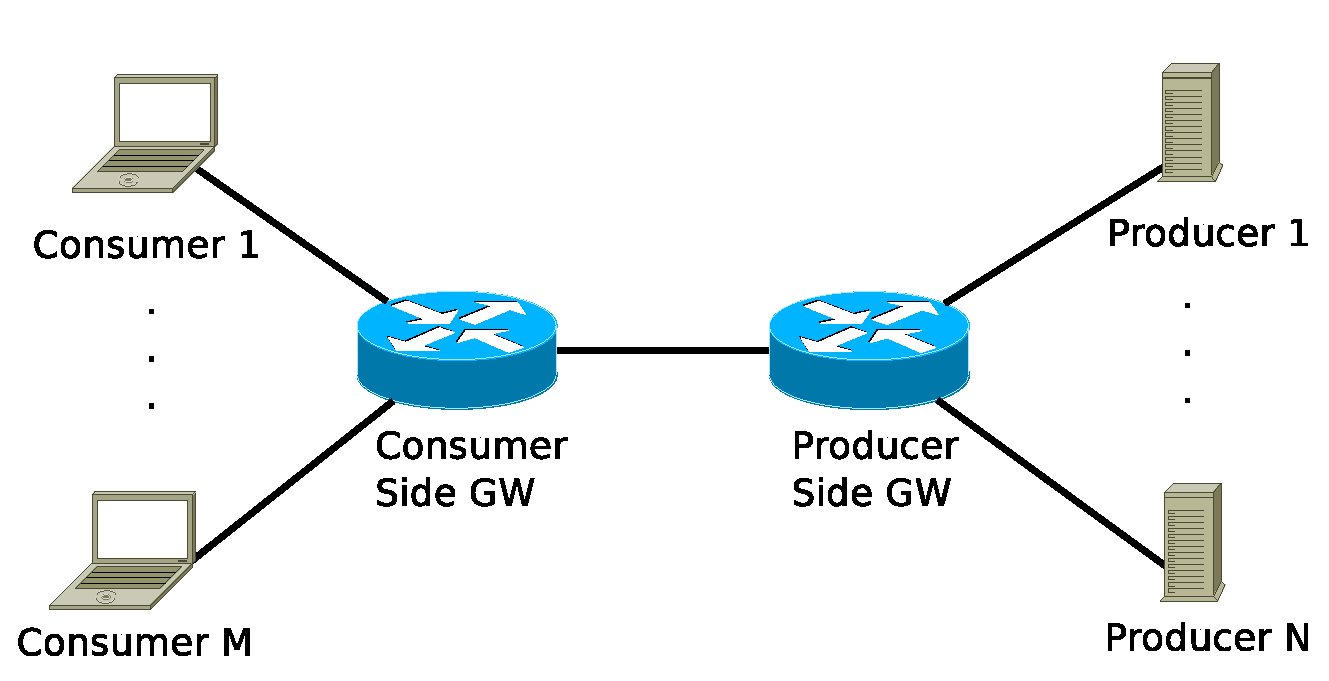
\includegraphics[width=\columnwidth]{images/testnet.eps}
\caption{Testbed network topology. $M$ consumers and $N$ producers}\label{testnet}
\end{figure}

CCVPN is implemented as a network layer service running on the gateways of the private networks that compose the VPN (see Fig.\ref{fig:ccvpn}).
Our implementation uses the CCNx software stack~\cite{CCNxGithub} and the cryptographic library Sodium~\cite{sodiumGithub}. These are both publicly available and written in C.
For the PKE version of CCVPN, we use Sodium Sealed-Boxes~\cite{bernstein2006curve25519}, implemented over X25519 elliptic curves, as the PKE algorithm for the interest encapsulation and decapsulation routines (Algorithm~\ref{alg:interestEncap}, and Algorithm~\ref{alg:interestDecap} of Sec.~\ref{metho}).
AES256-GCM~\cite{dworkin2007recommendation} is used to encrypt-then-MAC content responses (Alg.~\ref{alg:contentEnc}, and Alg.~\ref{alg:contentDec} of Sec.~\ref{metho}).
Recall that the symmetric keys used to encrypt-then-MAC the content packets are generated and sent together with the encapsulated interest in Alg.~\ref{alg:interestEncap}.
In the symmetric key version of the design, both, interests and contents, are encapsulated using AES256-GCM under the assumption that the gateways already share symmetric key.


The experiments presented throughout this section were executed in an Intel Core i7-3770 octacore CPU @3.40GHz, with 16GB of RAM, running Linux (Ubuntu 14.04LTS). Content payload sizes were set to 10 kilobytes.
On every experiment, each of the two gateway processes (i.e., consumer side gateway process, and producer side gateway process) were assigned as a high priority processes and each of them ran in a single core of the processor.
Table~\ref{should_be_figure} (\todo{Should be a single figure w/ six boxplots}) presents boxplots for the execution times of the four algorithms involved in CCVPN's data transmission, including both, PKE and Symm. Key versions for interest encapsulation and decapsulation.

\begin{table}[!h]
\centering
\caption{Interest encapsulation processing times}
\label{should_be_figure}
\begin{tabular}{|l|l|l|l|l|}
\hline
Encapsulation mode   & Encapsulation & Decapsulation \\ \hline
Public Key  & 444$\mu s$           & 449$\mu s$           \\ \hline \cline{4-5}
Symmetric Key & TODO          & TODO          \\ \hline
\end{tabular}
\end{table}

\begin{table}[!h]
\centering
\caption{Content encryption and decryption times for different payload sizes}
\label{my-label}
\begin{tabular}{|l|l|l|}
\hline
Packet size        & Encryption & Decryption \\ \hline
$1024$B & 125$\mu s$        & 193$\mu s$        \\ \hline
$4096$B & 141$\mu s$        & 220$\mu s$        \\ \hline
$16384$B & 220$\mu s$        & 367$\mu s$        \\ \hline
$65536$B & 519$\mu s$        & 702$\mu s$        \\ \hline
\end{tabular}
\end{table}

With the goal of evaluating the impact of CCVPN's cryptographic overhead on the overall network performance, we measure the network throughput and the request-response round trip time (RTT) under different topology settings.
In our testbed network, the consumers' side and the producers' side gateways are directly interconnected. $N$ producers are connected to the producers' domain gateway and $M$ consumers are connected to the consumers' domain gateway, as illustrated in Fig.~\ref{testnet}.
Under such topology we consider three variations for the values of ${M,N}$:

\begin{itemize}
 \item \textbf{One consumer and one producer $[1,1]$}:
 \item \textbf{Multiple consumers and one producer $[M,1]$}:
 \item \textbf{Multiple consumers and multiple producers $[M,N]$}:
\end{itemize}




To investigate the processing overhead we measure the average time demand for computing the interests' encapsulation (in public and symmetric key versions), interest decapsulation, content encryption, and content decryption for different content packet sizes (1024, 4096, 16384, and 65536 bytes). We also measure the state consumption for these same four functions.

To compute the overall network throughput we measure the average data-rate for transmissions of 1 to 1,000,000 different interests issues per consumer. We also vary the number of consumers and producers from 1 to 10 of each. Finally, in addition to the network throughput, we also exhibit the total transmission delay for each of the experiments.

\todo{TODO: Add results discussion}

\begin{figure}[]
\centering
  \subfigure[Throughput]{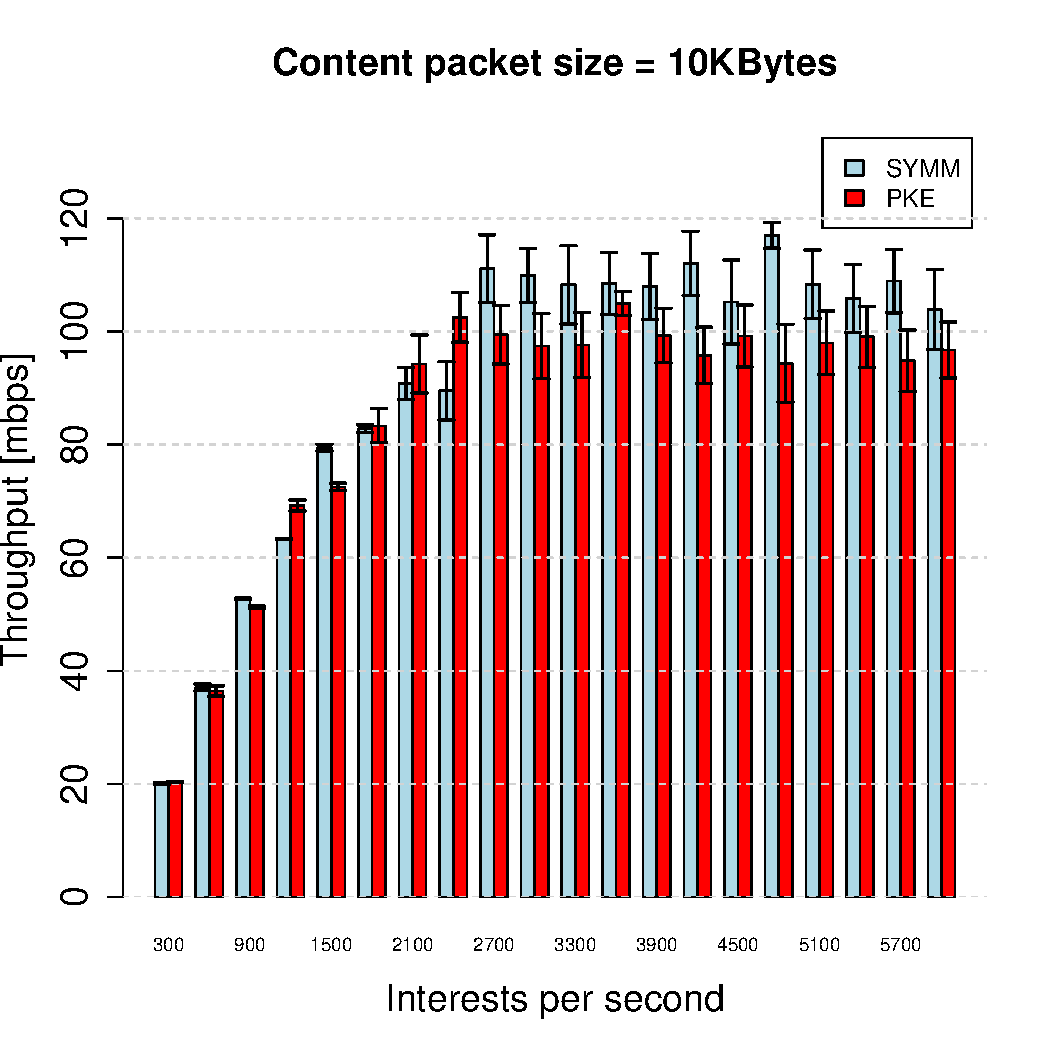
\includegraphics[width=0.8\columnwidth]{images/1_1_thput.pdf}\label{1a}}
  \hfil
  \subfigure[Avg. RTT]{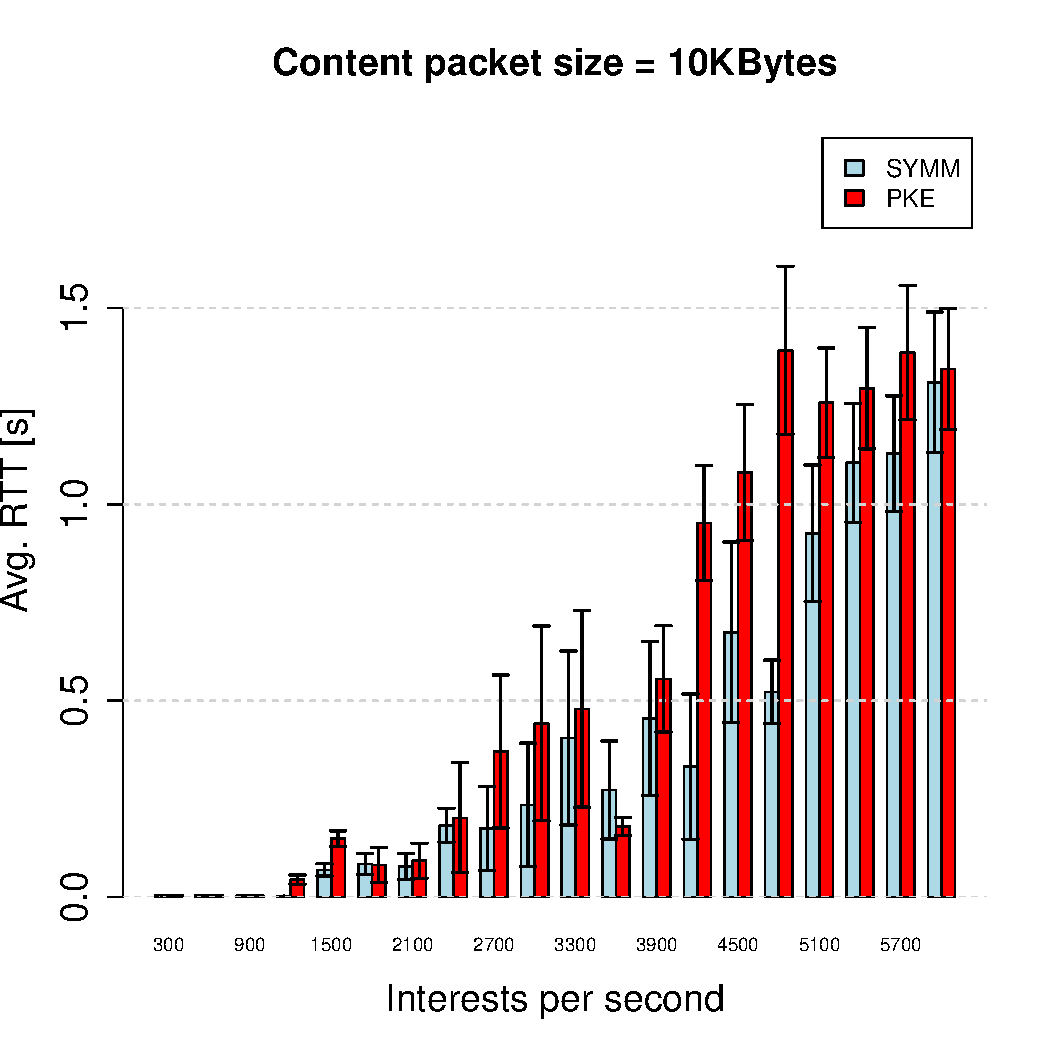
\includegraphics[width=0.8\columnwidth]{images/1_1_rtt.pdf}\label{1b}}
\caption{CCVPN performance with one consumer and one producer for increasing interest issuance rates.}\label{exp1}
\end{figure}

\begin{figure}[]
\centering
  \subfigure[Throughput]{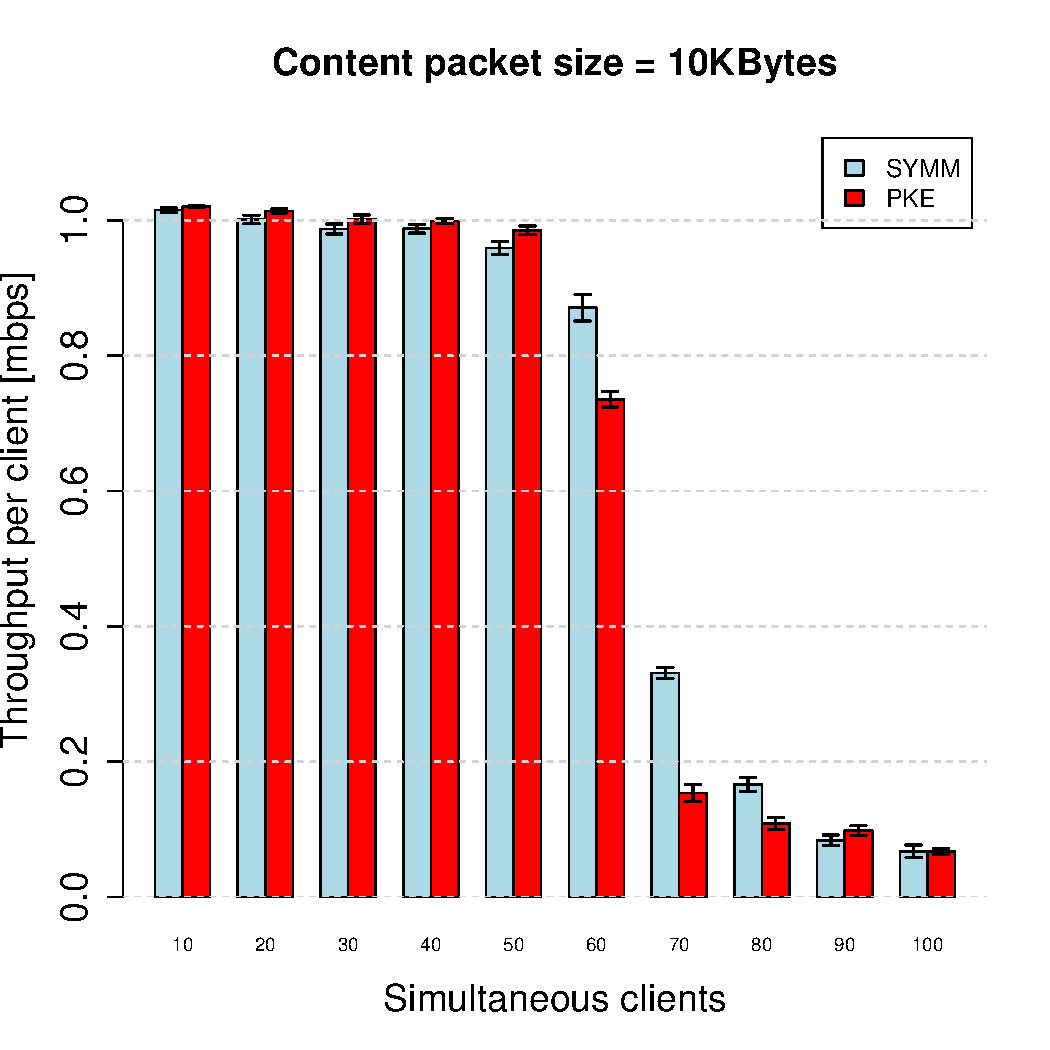
\includegraphics[width=0.8\columnwidth]{images/n_1_thput.pdf}\label{1a}}
  \hfil
  \subfigure[Avg. RTT]{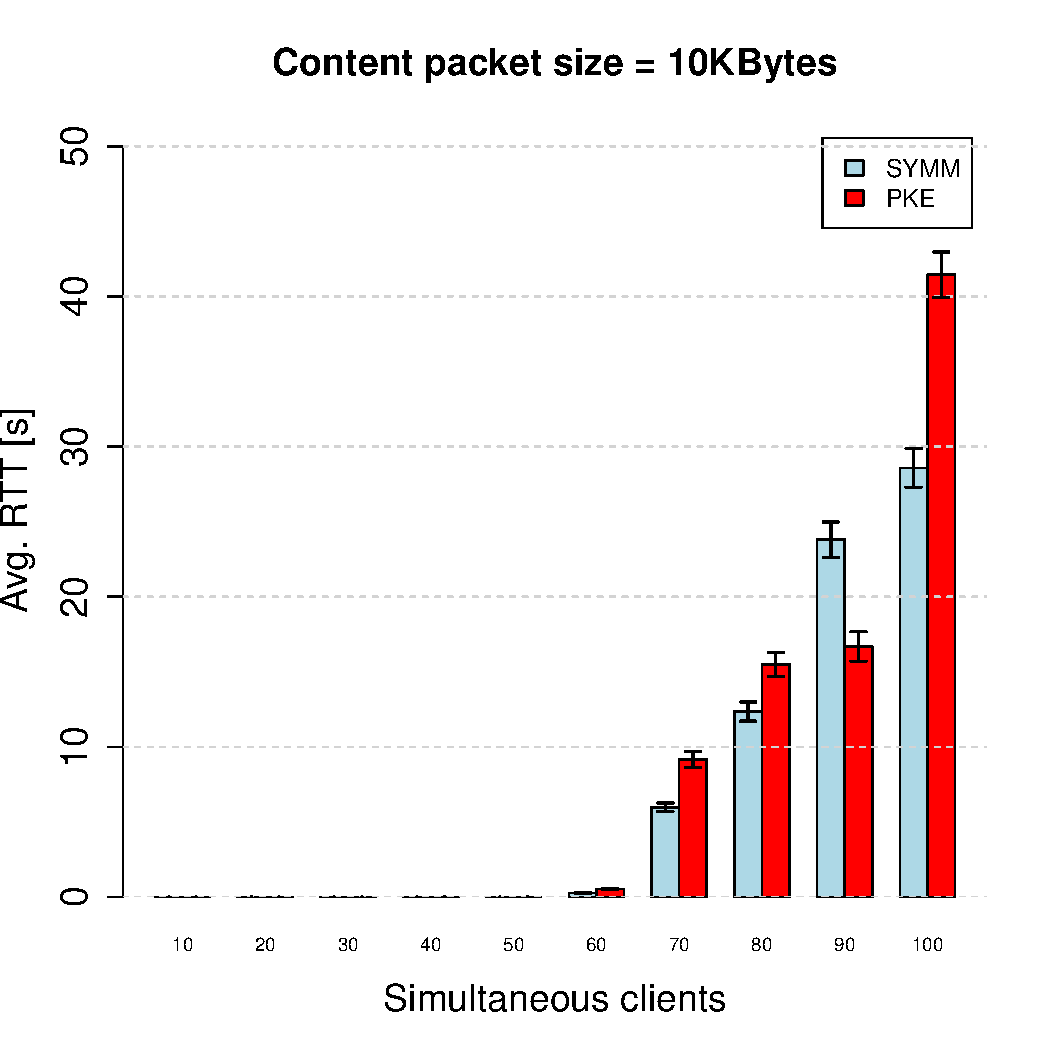
\includegraphics[width=0.8\columnwidth]{images/n_1_rtt.pdf}\label{1b}}
\caption{CCVPN performance with multiple consumers and one producer. Each consumer requests with 1 mbps rate.}\label{exp1}
\end{figure}

\begin{figure}[]
\centering
  \subfigure[Throughput]{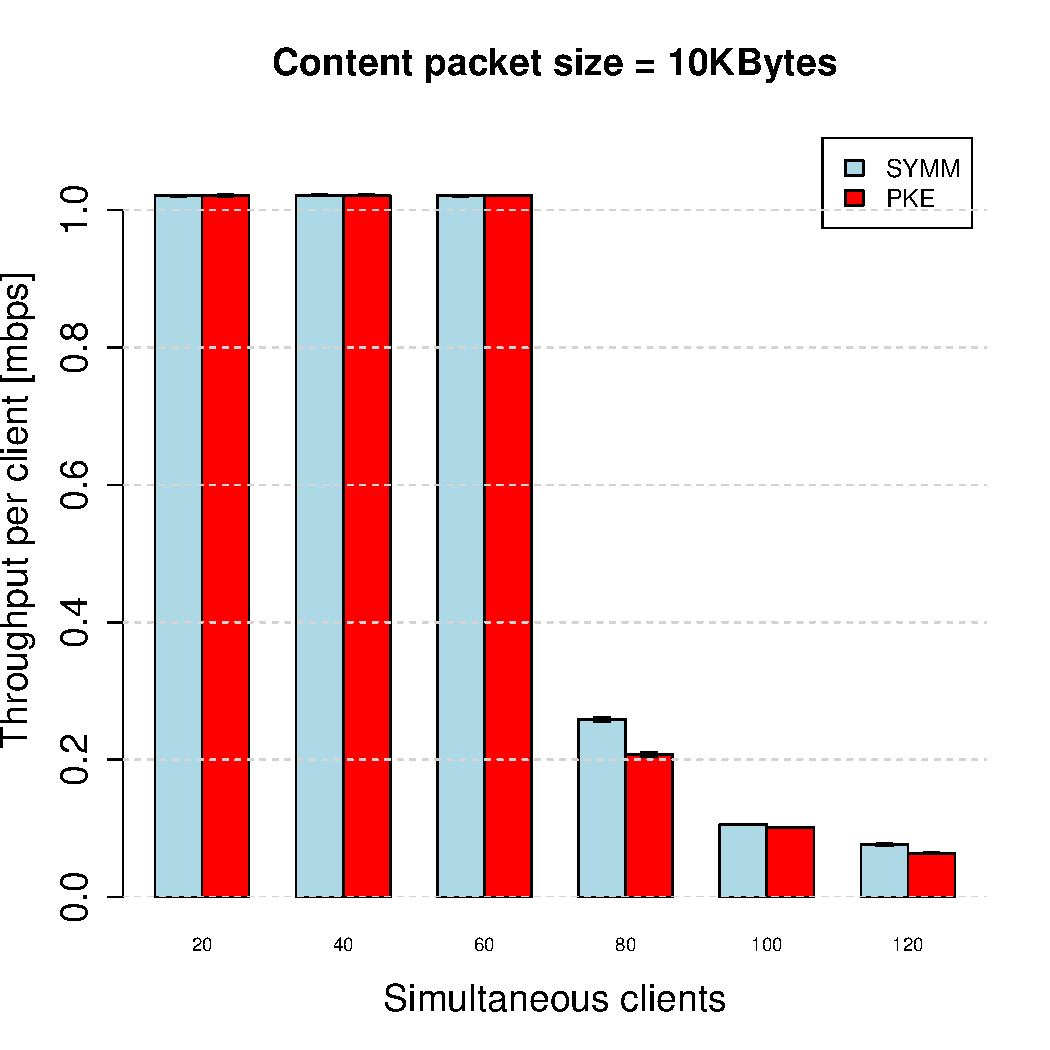
\includegraphics[width=0.8\columnwidth]{images/n_n_thput.pdf}\label{1a}}
  \hfil
  \subfigure[Avg. RTT]{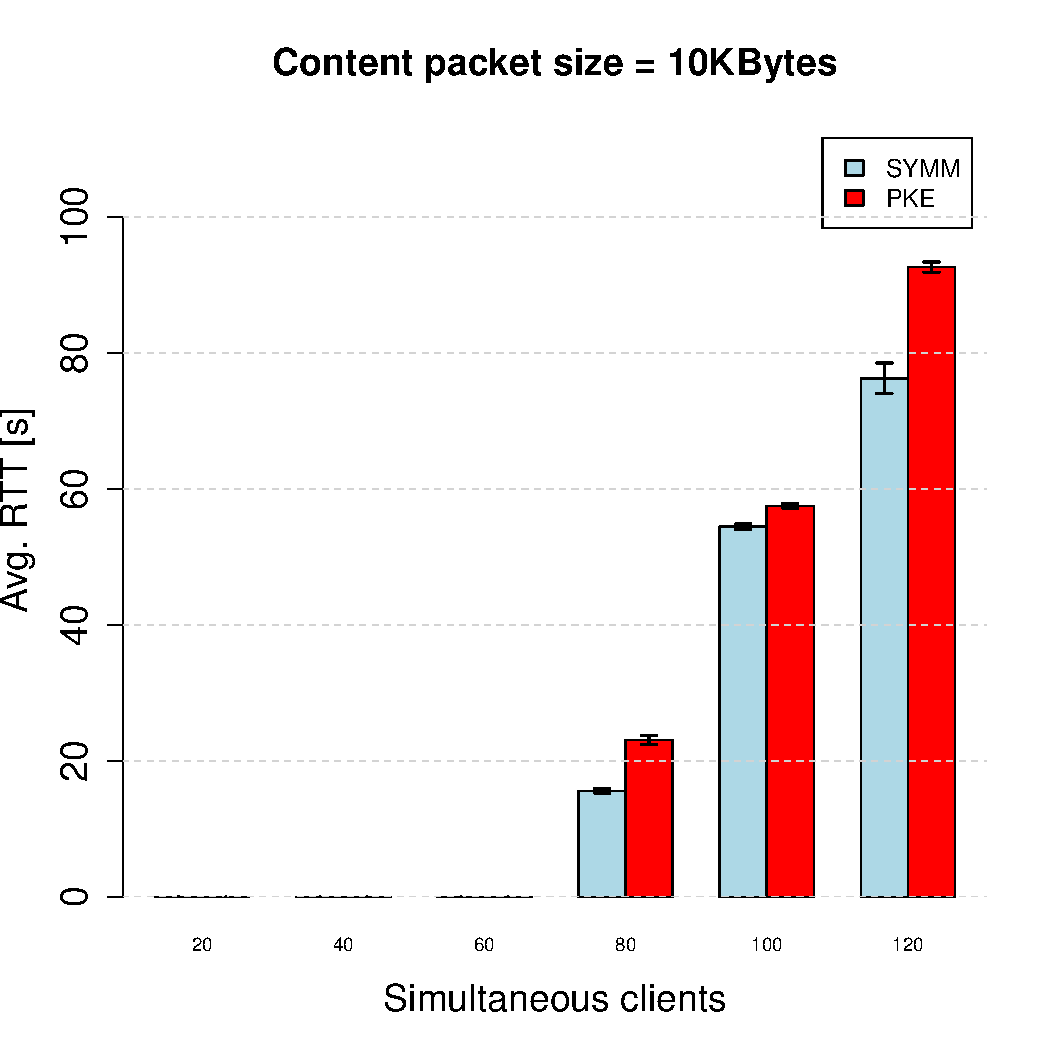
\includegraphics[width=0.8\columnwidth]{images/n_n_rtt.pdf}\label{1b}}
\caption{CCVPN performance with multiple consumers and multiple producers. Each consumer requests with 1 mbps rate.}\label{exp1}
\end{figure}


\section{Conclusion}\label{conclusion}
\todo{TODO}

\ifCLASSOPTIONcaptionsoff
  \newpage
\fi

\tiny

\bibliographystyle{IEEEtran}
\bibliography{references}

% \begin{IEEEbiography}[{\includegraphics[width=1in,height=1.25in,clip,keepaspectratio]{picture}}]{John Doe}
% \blindtext
% \end{IEEEbiography}

\end{document}
